\documentclass[runningheads]{llncs}

\usepackage{graphicx}
% Used for displaying a sample figure. If possible, figure files should
% be included in EPS format.
\usepackage{float}
\usepackage{appendix}

\begin{document}
	%
	\title{Scientific Paper}
	
	\author{Benjamin Vandersmissen\inst{1} \and
		Lars Van Roy\inst{2} \and \\
		Evelien Daems\inst{3} \and
		Frank Jan Fekkes\inst{4}}
	%
	\authorrunning{B. Vandersmissen, L. Van Roy, E. Daems, F.J. Fekkes}
	% First names are abbreviated in the running head.
	% If there are more than two authors, 'et al.' is used.
	%
	\institute{
		\email{benjamin.vandersmissen@student.uantwerpen.be} \and
		\email{lars.vanroy@student.uantwerpen.be} \and
		\email{evelien.daems@student.uantwerpen.be} \and
		\email{franciscus.fekkes@student.uantwerpen.be}}
	%
	\maketitle              % typeset the header of the contribution
	%
	\begin{abstract}
		This paper will give an in depth view of the performed adaptations to the Stride project, as well as an overview of the findings that were obtained by comparing these additions to the original stride project. 
		
		%\keywords{First keyword  \and Second keyword \and Another keyword.}
		
	\end{abstract}
	
	
	\section{Introduction}
	The stride project is designed to simulate and evaluate the lifetime of various infectious diseases. In order to properly analyze which factors have an effect on various diseases, the stride project allows multiple factors to be varied so that we can get an idea of which factors are the main influence  for the evolution of diseases. This expansion to the original stride project will include 2 major corrections, to make the simulation more realistic, being an improved workplace size distribution and an improved household composition distribution, a major addition to the pools in which diseases can spread, being daycare and preschool pools, a minor addition to make the input more variable by adding two addition input types being HDF5 and JSON and finally a visualizer that will allow users to get a graphical overview of where the diseases are most active, along with a list of parameters to give further information of the evolution of the disease for a given location. \\
	\\
	Other than these additions, there will also be a section about the simulation over entire Belgium, compared to isolated within Flanders. Other than just the simulated area, there will also be a comparison between the data derived from the Belgian population and the data derived from the Flemish population.
	
	\section{Daycare \& Preschool}
		In the original stride implementation, there are no specific contact pools for children aged 6 and under. The only way they could get infected was via the HouseHold contactpool. This is of course unrealistic. In this iteration of stride, 2 more contact pools are added, Daycare for children aged 0 to 3 and PreSchool for children aged 3 to 6. In this section, we discuss some of the repercussions of this change. \\ 
	\\
	Intuitively, by adding these contactpools, we should see that diseases spread faster than normal. To test this hypothesis, we generated a geopopulation with daycares and preschools and one without. Both are generated with the config file \textit{run\_generate\_default.xml} and then used them both in simulations.The result is shown in the following graph.
	\begin{figure}
			\centering
		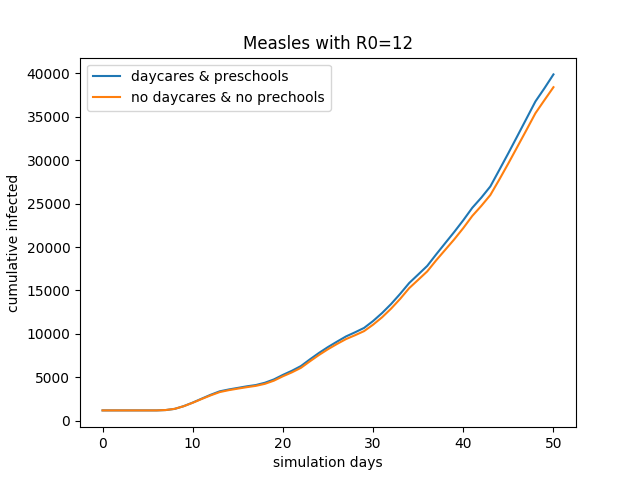
\includegraphics[width=0.9\textwidth]{measles_r12_daycare_comparison.png}	
		\caption{Average result of 10 simulations with and without daycares and preschools}
		\label{fig0}
	\end{figure}
	\\
	As shown in the graph, there are more infected persons with the implementation of daycares and preschools. With these parameters, there are around 2000 infected more after 50 days or a little more than 5\% extra infected.
	\section{Data Formats}
	\subsection{JSON}
	\subsection{HDF5}
	HDF5 is a scientific dataformat specifically designed to store and organise large amounts of data. In this section, we compare the sizes of the fileformats already available in stride (protobuf and JSON) with the size of an HDF5 file and we also cover the write speed. Both these metrics are based on the configuration file \textit{run\_generate\_default.xml} with only the output file changed.
	\\
	As shown in table \ref{table:1}, HDF5 is memory-wise between protobuf and JSON. This is because protobuf is a heavily compressed format and HDF5 is not, but HDF5 isn't a plain text format like JSON either. In terms of write speed, HDF5 is a lot slower than Protobuf and JSON. A simple explanation for this is the fact that HDF5 does not support streams, while JSON and Protobuf do. This means that HDF5 has to write everything with it's own procedures which isn't as efficient. HDF5 does not support streams, because it was originally a C library, where streams did not exist and the C++ implementation is just a wrapper around the original C library.
	\begin{table}
		\centering
		\begin{tabular}{|c|c|c|}
			\hline
			\textbf{FileFormat} & \textbf{Size (Kb)}  & \textbf{Average write Time (s)}\\ \hline
			Protobuf & 13.713 & 1.74\\ \hline
			JSON & 317.050 & 5.25\\ \hline
			HDF5 & 125.066 & 30.45 \\ \hline
		\end{tabular}
		\caption{Performance of different data formats based on 10 runs of run\_generate\_default.xml}
		\label{table:1}
	\end{table}
	\section{Data Visualization}
	\section{Workplace Size Distribution}
	\subsection{Introduction}
	The original stride project made use of a set workplace size distribution, being an average size of 20, that would be randomly populated. So it might be that there would be smaller and larger workplaces, but the average would be around 20, which is not accurate. The majority of the workplaces are smaller than 20 and there are workplaces that are way larger than 20. It would therefore be more accurate to add an input file that would give a distribution of which workplace size occurs with which chance.

	\subsection{Impact}
	To proof whether or not this addition had a major impact, and to show the size of its impact, we ran a couple of simulations with different values for r0. The resulting graphs are displayed in the annex. Even though the difference isn't huge, we can generally conclude that it most definitely made the spreading go faster. At the end of the simulations, the number of infected people is generally about 4\% lower compared to using the newer workplace implementation. We can therefore conclude that the original workplace implementation was indeed incorrect, and gave slightly flawed results.
	\section{Household Composition Distribution}
	\subsection{Introduction}
	One more flaw of the original stride project, is that it had no regard for the differences in household size within smaller regions. It used one big input file, that would give the general household configuration over the entire simulation area (in this case Flanders) but there are significant differences between households over the different provinces. We therefore wanted to be able to specify household information for each province. \\
	\\
	Other than provinces, there are also significant differences between regular cities and major cities. We therefore added one extra household configuration for major cities, along with a file specifying which cities are considered to be major.
	\subsection{impact}
	To proof the impact of this addition, we did the same simulations we did for the workplace distribution addition. These plots, found in the annex, are different to the plots from workplaces in that they are not consistent in the effect that occurred. We can see significant effects in all three plots, but for r0 equal to 8 we see that the new implementation gives a far lower number of diseased people, where the other two show that the new implementation gives a slightly higher number of diseased people, compared to the original stride, spread over the two, the average is still a drop of 2\%. We can conclude that this change was significant and that there was indeed a flaw in the original stride implementation or, in other words, the differences between regions and cities are significant to the simulation.
	\section{Belgian Simulations}
	
	\newpage
	\appendix
	\appendixpage
	\section{Workplace Size Distribution}
	\begin{figure}
		\centering
		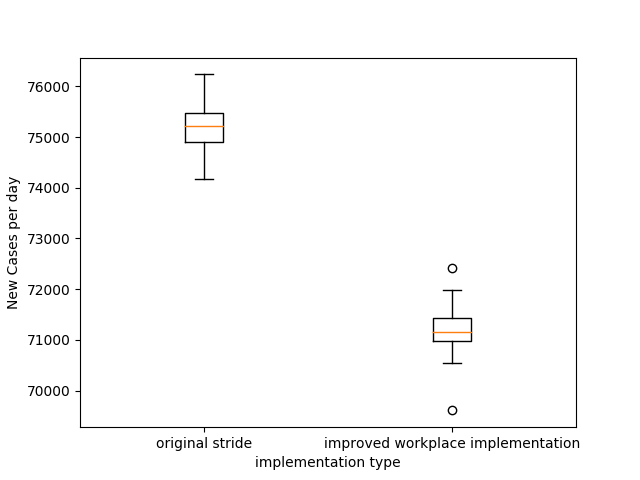
\includegraphics[width=0.9\textwidth]{workplace_r08_boxplot.png}	
		\caption{The boxplot for the different workplace implementations, using r0 equal to 8}
		\label{fig1}
	\end{figure}
	\begin{figure}
		\centering
		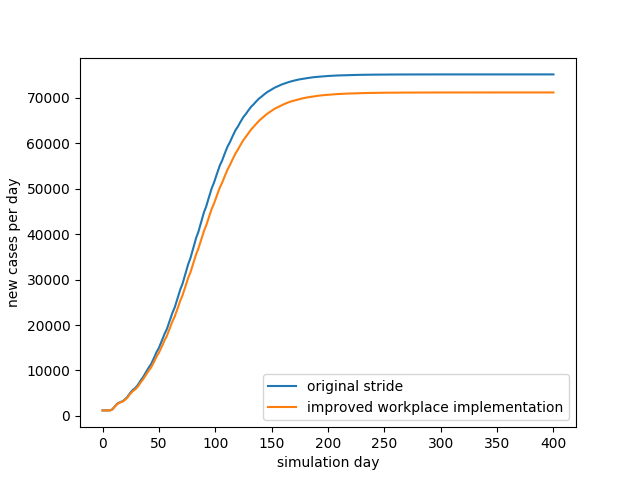
\includegraphics[width=0.9\textwidth]{workplace_r08_cumul.png}
		\caption{The cumulative evolution of the diseased people, using the different workplace implementations and r0 equal to 8}	
		\label{fig2}
		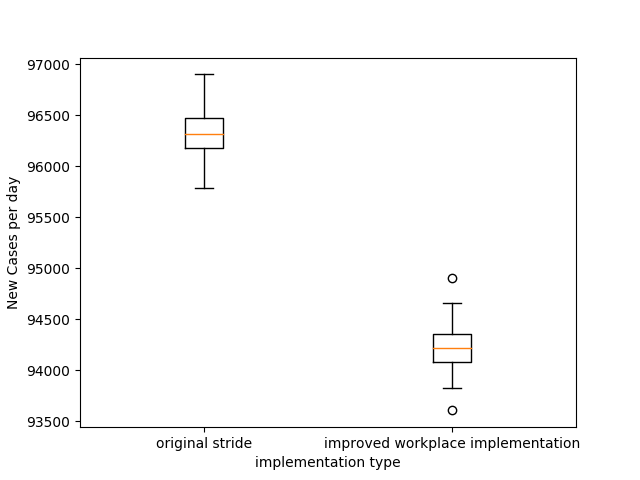
\includegraphics[width=0.9\textwidth]{workplace_r11_boxplot.png}	
		\caption{The boxplot for the different workplace implementations, using r0 equal to 11}
		\label{fig3}
	\end{figure}
	\begin{figure}
		\centering
		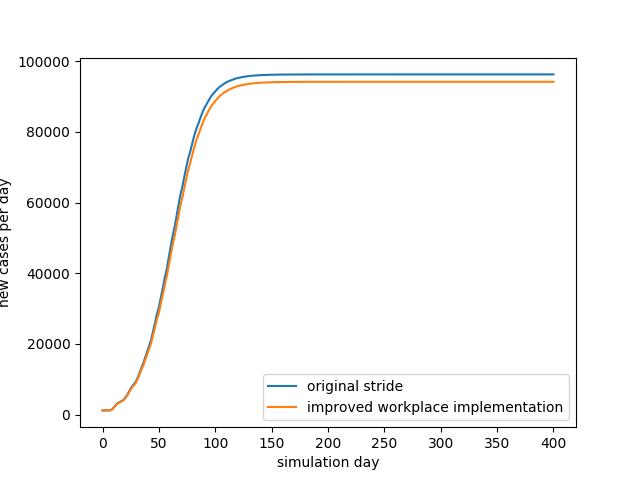
\includegraphics[width=0.9\textwidth]{workplace_r11_cumul.png}
		\caption{The cumulative evolution of the diseased people, using the different workplace implementations and r0 equal to 11}	
		\label{fig4}
		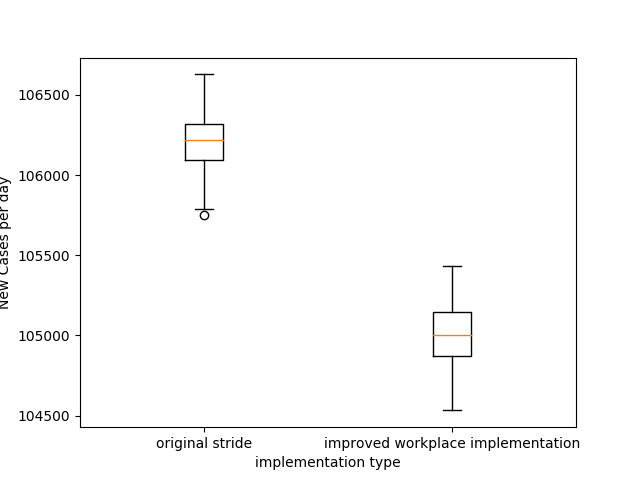
\includegraphics[width=0.9\textwidth]{workplace_r14_boxplot.png}	
		\caption{The boxplot for the different workplace implementations, using r0 equal to 14}
		\label{fig5}
	\end{figure}
	\begin{figure}
		\centering
		\centering
		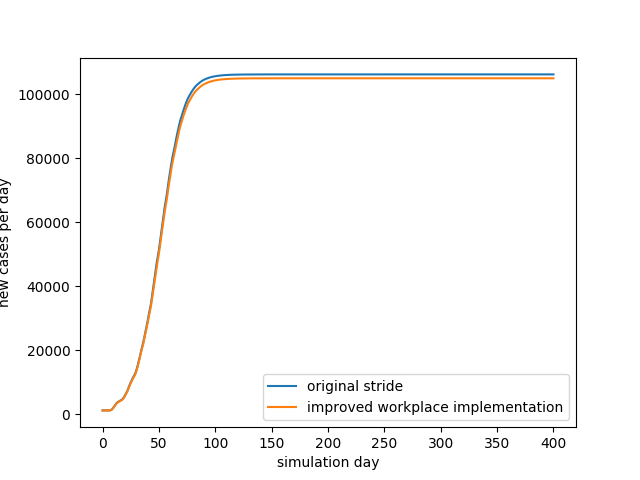
\includegraphics[width=0.9\textwidth]{workplace_r14_cumul.png}
		\caption{The cumulative evolution of the diseased people, using the different workplace implementations and r0 equal to 14}	
		\label{fig6}
	\end{figure}
	\clearpage
	\section{Household Composition Distribution}
	\begin{figure}
		\centering
		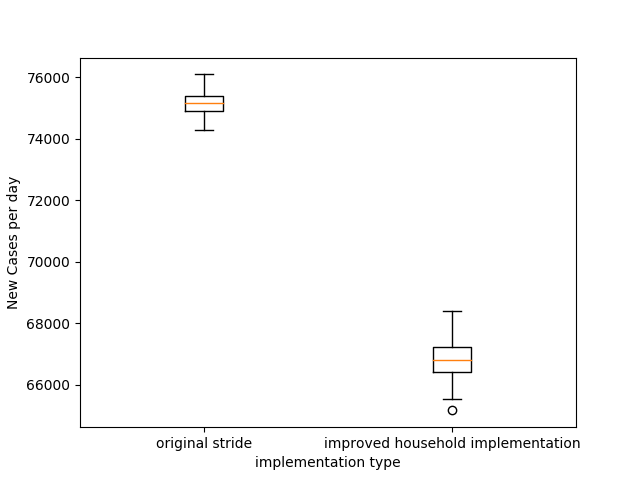
\includegraphics[width=0.9\textwidth]{household_r08_boxplot.png}	
		\caption{The boxplot for the different household implementations, using r0 equal to 8}
		\label{fig7}
	\end{figure}
	\begin{figure}
		\centering
		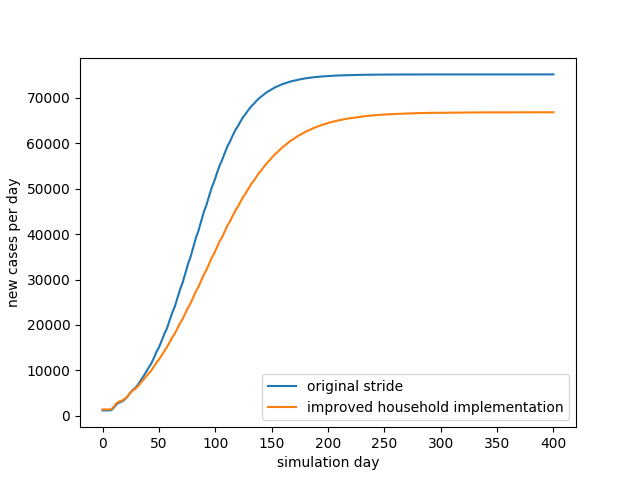
\includegraphics[width=0.9\textwidth]{household_r08_cumul.png}
		\caption{The cumulative evolution of the diseased people, using the different household implementations and r0 equal to 8}	
		\label{fig8}
		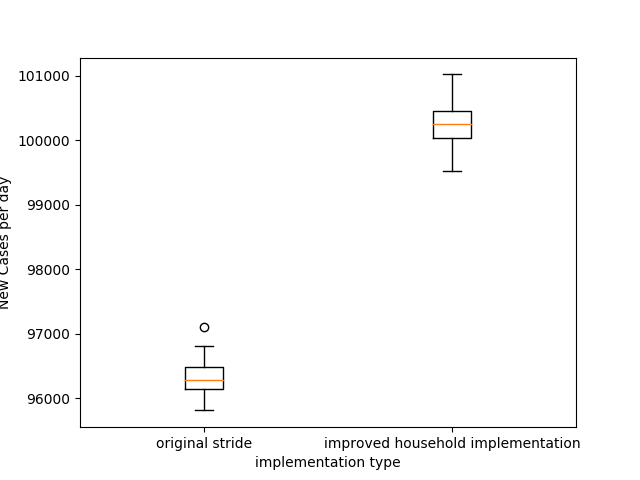
\includegraphics[width=0.9\textwidth]{household_r11_boxplot.png}	
		\caption{The boxplot for the different household implementations, using r0 equal to 11}
		\label{fig9}
	\end{figure}
	\begin{figure}
		\centering
		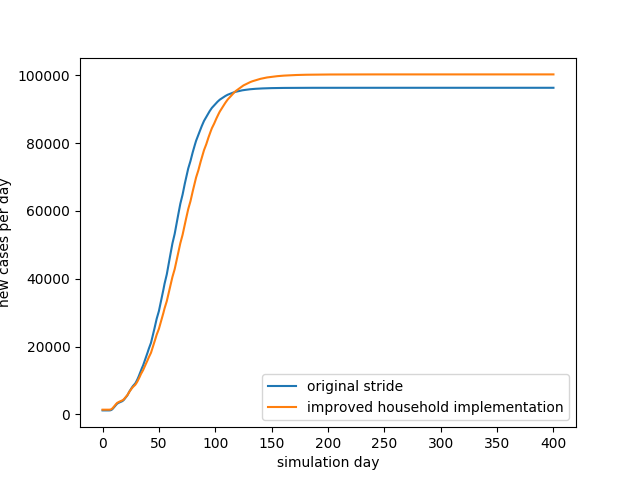
\includegraphics[width=0.9\textwidth]{household_r11_cumul.png}
		\caption{The cumulative evolution of the diseased people, using the different household implementations and r0 equal to 11}	
		\label{fig10}
		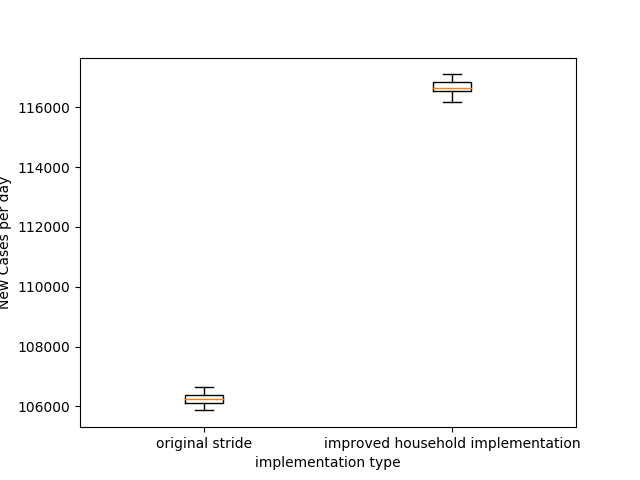
\includegraphics[width=0.9\textwidth]{household_r14_boxplot.png}	
		\caption{The boxplot for the different household implementations, using r0 equal to 14}
		\label{fig11}
	\end{figure}
	\begin{figure}
		\centering
		\centering
		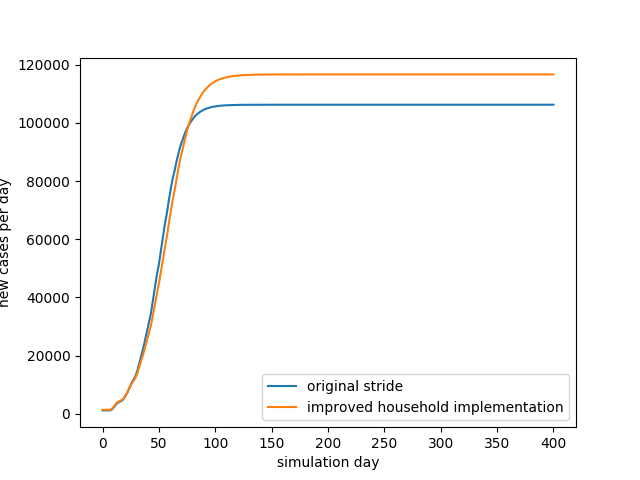
\includegraphics[width=0.9\textwidth]{household_r14_cumul.png}
		\caption{The cumulative evolution of the diseased people, using the different household implementations and r0 equal to 14}	
		\label{fig12}
	\end{figure}
\end{document}

